\documentclass{article}
\usepackage{graphicx}

\begin{document}
\title{Visual Tweets Sentimental Analysis}
\author{Lilong Jiang (jiang.573)}
\maketitle

\section{Introduction}
In this project, I build a visual online tweets sentimental analysis tool, which allows users to do the sentimental analysis for a certain topic. The user interface is shown in Figure 1. We implement two classifiers and compare the performance and accuracy in both classifiers. 
\section{Dataset}
We get our datset from the Sentiment140 \footnote{\texttt{\scriptsize{http://www.sentiment140.com/‎}}}. The training dataset in this dataset is collected by the Twitter API, whose content contains the emoticons. The test dataset in this dataset is manually annotated.
\section{Preprocessing}
There are several challenges for the tweets processing: firstly, the tweets are very short, limited as 140 characters. Secondly, the tweets are very sloppy and it contains a lot of misspellings, slangs, abbreviations and emoticons. The preprocessing step is very important for the later classification.
We preprocess all the tweets as follows: \\
(1) Remove usernames and urls. \\
(2) I use an emoticon dictionary ~\cite{agarwal2011sentiment}, in which each emoticon is labeled as emotion(positive or negative). The emoticons in the tweets are replaced by happy or sad. \\
(3) Replace all sequences of repeated characters by three characters, for example, convert goooood to goood.\\
(4) Expand abbreviations with a dictionary\footnote{\texttt{\scriptsize{http://www.noslang.com/‎‎}}}. For example, lol is converted into laughing out loud. \\
(4) NLTK\footnote{\texttt{\scriptsize{http://www.nltk.org/‎‎}}} is used to tokenize the tweets, remove the stop words, punctuations, and lemmatization. \\
(5) PyEnchant\footnote{\texttt{\scriptsize{http://pythonhosted.org/pyenchant/‎‎}}} is used to check whether the token is a correct English word. \\ 
\section{Classifiers}
We use two classifiers in this project. One is the naive Bayes classifier and the other is the SVM. 
\subsection{Naive Bayes Classifier}
The Naive Bayes classifier is a simple probalistic classifier which is based on Bayes theorem. Each tweet will be classified into the class with the highest posterior probability. \\
$C_{map} = argmax_{c \in C} (log P(c) + \sum_{1 \ge k \le n_d log P(t_k |c)})$\\
The conditional probability of a particular word given a class as the relative frequency of term t in documents belongs to class c:\\
$P(t|c) = \frac{T_{ct} + 1}{\sum_{t \in V}(T_{ct} + 1)} = \frac{T_{ct} + 1}{\sum_{t \in V}(T_{ct}) + B}$ \\
where B is the number of documents. \\
We use add-one smoothing to address the problem that a particular word doesn't appear in a particular class.
\subsection{Feature Selection}
I implement two feature selection methods. One is the frequency-based feature selection. The other is based on the mutual information.
\subsubsection{Frequency-based Feature Selection}
\subsubsection{Mutual Information}
Mutual INformation is used to measure how much a term t contributes to the class c. \\
$I(U; C) = \frac{N_{11}}{N} \log_2 \frac{N N_{11}}{N_{1.}N_{.1}} + \frac{N_{01}}{N} \log_2 \frac{N N_{01}}{N_{0.}N_{.1}} + \frac{N_{10}}{N} \log_2 \frac{N N_{10}}{N_{1.}N_{.0}} + \frac{N_{00}}{N}\log_2 \frac{N N_{00}}{N_{0.}N_{.0}}$\\
where $N_{10}$ is the number of documents that contain t and are not in class c. $N_{11}$ is the number of documents that contain t and are in class c. $N_{01}$ is the number of documents that dont contain t and are in class c. $N_{00}$ is the number of documents that dont contain t and are not in class c. $N_{1.}$ is the number of documents that contain t. $N_{1.}$ is the number of documents that contain t. \\
We use add-1 smoothing for each count to void the divided by 0.
\subsection{SVM Classifier}
We use Libsvm\footnote{\texttt{\scriptsize{http://www.csie.ntu.edu.tw/~cjlin/libsvm//‎‎}}} to classify the tweets. ‎
\subsection{Experiment}
We compare these two classifier on the performance and accuracy. 2000 tweets are used to train the classifers (1000 tweets are positive and 1000 tweets are negative) and 359 tweets are used to test the classifier.
\subsubsection{Parameter Sensitivity}
Shrinking Size \\
We plot the accuracy of Bayes classifier with the changing of the shrinking ratio in the mutual information. The result is shown in Figure. As we can see 
\subsubsection{Performance}
\subsubsection{Accuracy}
\section{Online Sentimental Analysis}
\subsection{Architecture}
\begin{figure}
\centering
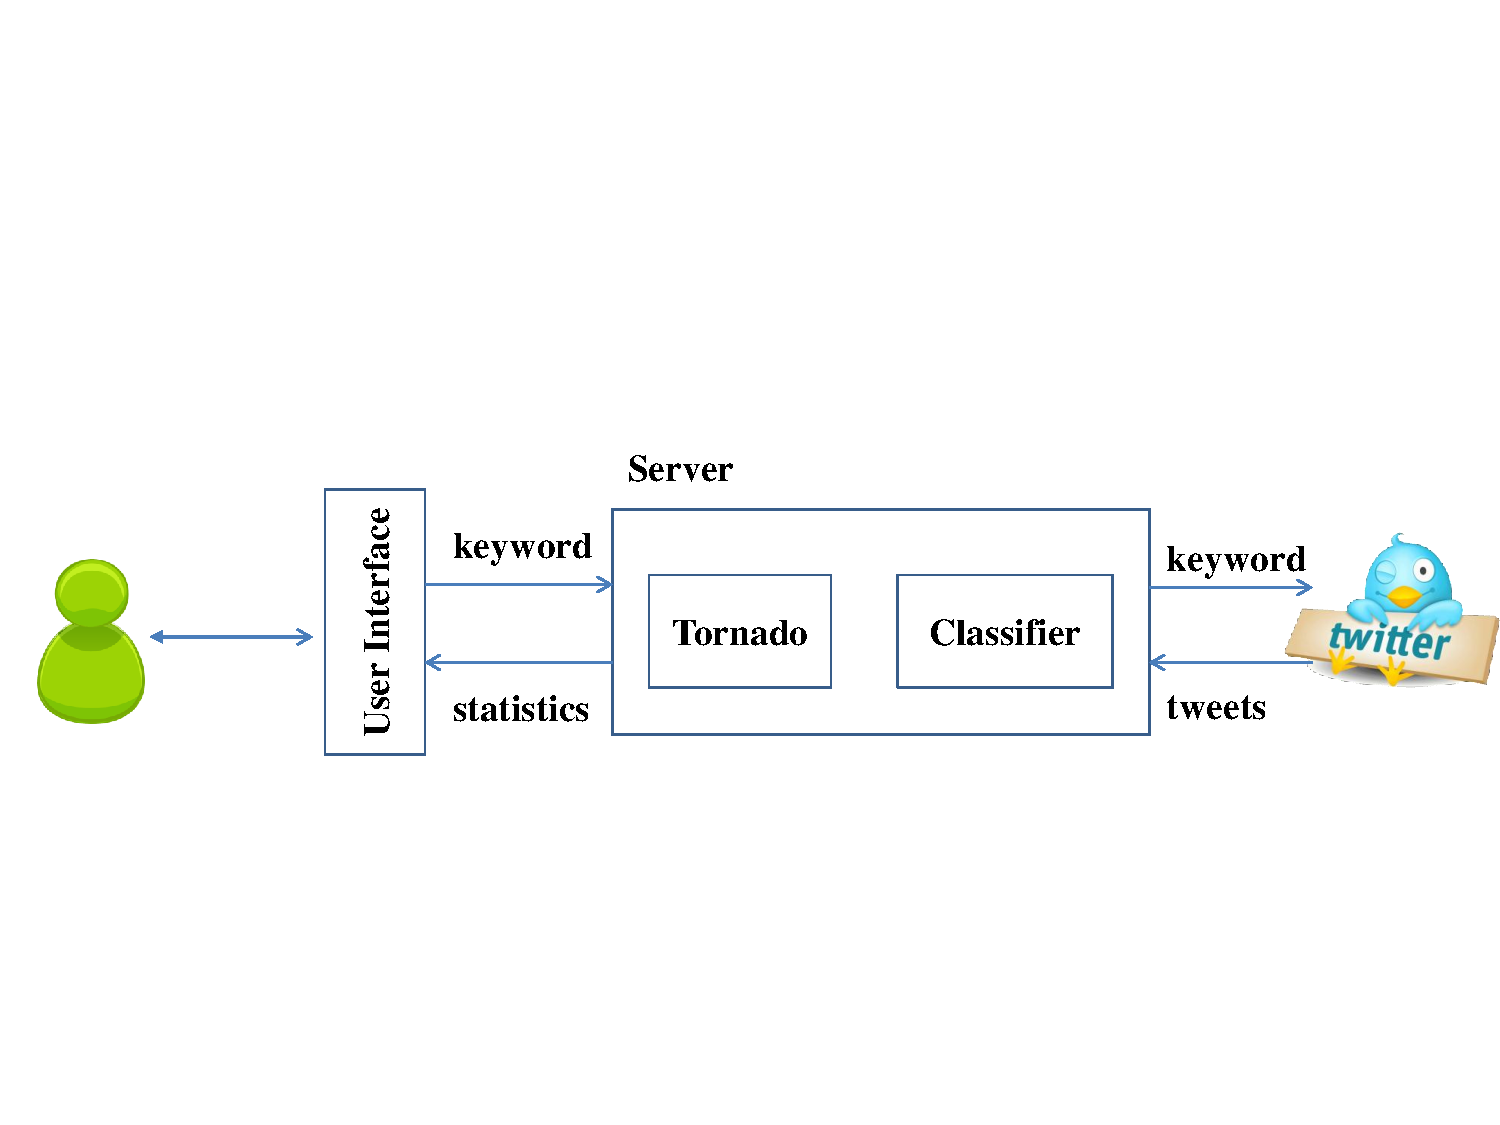
\includegraphics[width=0.8\textwidth]{pics/architecture}
\caption{Architecture}
\label{Fig:architecture}
\end{figure}
In the front end, we use d3\footnote{\texttt{\scriptsize{http://d3js.org/‎‎}}} to visualize the final result and Tornado\footnote{\texttt{\scriptsize{http://www.tornadoweb.org/}}} as a webserver. When users submit a topic, the server gets 1000 tweets from the twitter through twitter api and analyzes each tweet and returns the statistics information and tweets to the client. 
\subsection{Data Collection}
TwitterSearch\footnote{\texttt{\scriptsize{http://twittersearch.readthedocs.org/en/latest//‎‎}}} is a python-based interface which implements the Twitter Search API. 
\subsection{Online Analysis}
\end{document}
